\chapter{Sensores de Presión}
La presión es una fuerza por unidad de superficie y puede expresarse en unidades tales como Pascal (S.I.), bar, atmósferas, kilogramos por centímetro cuadrado y psi (libras por pulgada cuadrada).

\begin{figure}[H]
    \centering
    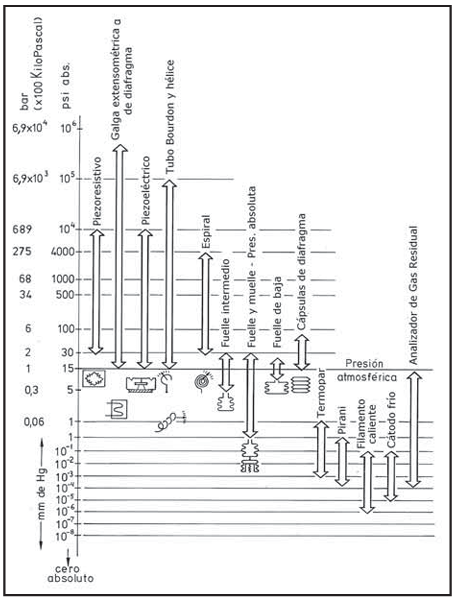
\includegraphics[width=0.5\linewidth]{Imagenes/Presion.png}
    \caption{Instrumentos de presión y campo de aplicación}
\end{figure}

Las clases de presión absoluta o diferencial que los instrumentos miden comúnmente en la industria son:
\begin{itemize}
    \item \textit{Presión absoluta} que se mide con relación al cero absoluto de presión.
    \item \textit{Presión atmosférica} es la presión ejercida por la atmósfera terrestre a nivel del mar medida mediante un barómetro.
    \item \textit{Presión relativa}, que es la diferencia entre la presión absoluta y la atmosférica del lugar donde se realiza la medición.
    \item \textit{Presión diferencial} es la diferencia entre dos presiones.
    \item \textit{Vacío} es la diferencia de presiones entre la presión atmosférica existente y la presión absoluta, es decir, es la presión medida por debajo de la atmosférica.
\end{itemize}

\section{Elementos mecánicos}
Podemos dividirlos en elementos primarios de medida directa que miden la presión comparándola con la ejercida por un líquido de densidad y altura conocidas (barómetro cubeta, manómetro de tubo en U, manómetro de tubo inclinado, manómetro de toro pendular, manómetro de campana) y en elementos primarios elásticos que se deforman con la presión interna del fluido que contienen.

Los elementos primarios elásticos más empleados son el tubo de Bourdon, el elemento en espiral, el helicoidal, el diafragma y el fuelle.

Los materiales empleados normalmente son acero inoxidable, aleación de cobre o níquel o aleaciones especiales como hastelloy y monel.

\section{Elementos electromecánicos}
Los elementos electromecánicos de presión utilizan un elemento mecánico combinado con un transductor eléctrico, que genera la correspondiente señal eléctrica. Se clasifican según el principio de funcionamiento en los siguientes tipos: resistivos, magnéticos, capacitivos, extensométricos y piezoeléctricos.

Los elementos resistivos están constituidos de un elemento elástico que varía la resistencia óhmica de un potenciómetro en función de la presión.

Los elementos de inductancia variable utilizan el transformador diferencial variable lineal que proporciona una señal en c.a. proporcional al movimiento de una armadura de material magnético situada dentro de un imán permanente o una bobina que crea un campo magnético.

Los elementos de reluctancia variable se basan en el desplazamiento mecánico, debido a la presión, de un núcleo magnético situado en el interior de una o dos bobinas.

Los elementos capacitivos se basan en la variación de capacidad que se produce en un condensador al desplazarse una de sus placas por la aplicación de presión.

Los elementos de galgas extensiométricas se basan en la variación de longitud y de diámetro, y por lo tanto de resistencia, que tiene lugar cuando un hilo de resistencia se encuentra sometido a una tensión mecánica por la acción de una presión.

Los elementos piezoeléctricos son materiales cristalinos que, al deformarse físicamente por la acción de una presión, generan un potencial eléctrico. Dos materiales típicos en los transductores piezoeléctricos son el cuarzo y el titanato de bario, capaces de soportar temperaturas del orden de 150ºC en servicio continuo y de 230ºC en servicio intermitente.

Los elementos de película delgada son sensores piezoresistivos, adecuados para presiones superiores a 25 bar, que consisten en membranas cubiertas con una capa de resistencia, cuyo valor cambia con la aplicación de presión.

\section{Elementos electrónicos de vacío}
Los elementos electrónicos de vacío se emplean para la medida de alto vacío, son muy sensibles y se clasifican en los siguientes tipos:
\begin{itemize}
    \item Medidos McLeod
    \item Mecánicos - Tubo Bourdon, fuelle y diafragma.
    \item Propiedades de un gas - Conductividad térmica.
    \item Térmicos - Termopar, Pirani, bimetal.
    \item Ionización - Filamento caliente, cátodo frío.
\end{itemize}

\begin{figure}[H]
    \centering
    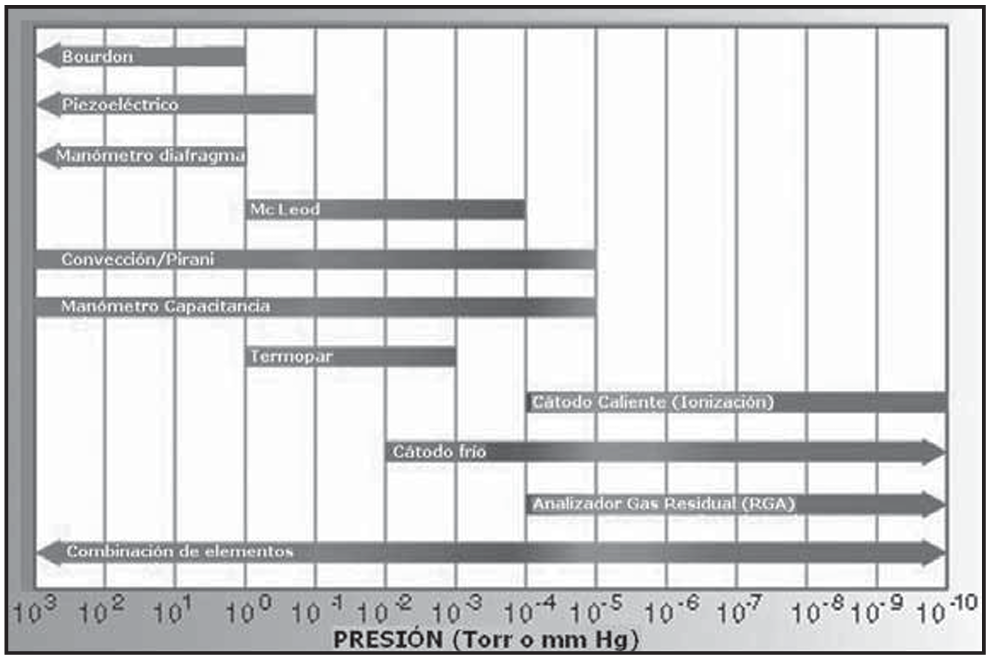
\includegraphics[width=0.5\linewidth]{Imagenes/Presion2.png}
    \caption{Campos de trabajo de los elementos electrónicos de vacío.}
\end{figure}